\documentclass[1p]{elsarticle_modified}
%\bibliographystyle{elsarticle-num}

%\usepackage[colorlinks]{hyperref}
%\usepackage{abbrmath_seonhwa} %\Abb, \Ascr, \Acal ,\Abf, \Afrak
\usepackage{amsfonts}
\usepackage{amssymb}
\usepackage{amsmath}
\usepackage{amsthm}
\usepackage{scalefnt}
\usepackage{amsbsy}
\usepackage{kotex}
\usepackage{caption}
\usepackage{subfig}
\usepackage{color}
\usepackage{graphicx}
\usepackage{xcolor} %% white, black, red, green, blue, cyan, magenta, yellow
\usepackage{float}
\usepackage{setspace}
\usepackage{hyperref}

\usepackage{tikz}
\usetikzlibrary{arrows}

\usepackage{multirow}
\usepackage{array} % fixed length table
\usepackage{hhline}

%%%%%%%%%%%%%%%%%%%%%
\makeatletter
\renewcommand*\env@matrix[1][\arraystretch]{%
	\edef\arraystretch{#1}%
	\hskip -\arraycolsep
	\let\@ifnextchar\new@ifnextchar
	\array{*\c@MaxMatrixCols c}}
\makeatother %https://tex.stackexchange.com/questions/14071/how-can-i-increase-the-line-spacing-in-a-matrix
%%%%%%%%%%%%%%%

\usepackage[normalem]{ulem}

\newcommand{\msout}[1]{\ifmmode\text{\sout{\ensuremath{#1}}}\else\sout{#1}\fi}
%SOURCE: \msout is \stkout macro in https://tex.stackexchange.com/questions/20609/strikeout-in-math-mode

\newcommand{\cancel}[1]{
	\ifmmode
	{\color{red}\msout{#1}}
	\else
	{\color{red}\sout{#1}}
	\fi
}

\newcommand{\add}[1]{
	{\color{blue}\uwave{#1}}
}

\newcommand{\replace}[2]{
	\ifmmode
	{\color{red}\msout{#1}}{\color{blue}\uwave{#2}}
	\else
	{\color{red}\sout{#1}}{\color{blue}\uwave{#2}}
	\fi
}

\newcommand{\Sol}{\mathcal{S}} %segment
\newcommand{\D}{D} %diagram
\newcommand{\A}{\mathcal{A}} %arc


%%%%%%%%%%%%%%%%%%%%%%%%%%%%%5 test

\def\sl{\operatorname{\textup{SL}}(2,\Cbb)}
\def\psl{\operatorname{\textup{PSL}}(2,\Cbb)}
\def\quan{\mkern 1mu \triangleright \mkern 1mu}

\theoremstyle{definition}
\newtheorem{thm}{Theorem}[section]
\newtheorem{prop}[thm]{Proposition}
\newtheorem{lem}[thm]{Lemma}
\newtheorem{ques}[thm]{Question}
\newtheorem{cor}[thm]{Corollary}
\newtheorem{defn}[thm]{Definition}
\newtheorem{exam}[thm]{Example}
\newtheorem{rmk}[thm]{Remark}
\newtheorem{alg}[thm]{Algorithm}

\newcommand{\I}{\sqrt{-1}}
\begin{document}

%\begin{frontmatter}
%
%\title{Boundary parabolic representations of knots up to 8 crossings}
%
%%% Group authors per affiliation:
%\author{Yunhi Cho} 
%\address{Department of Mathematics, University of Seoul, Seoul, Korea}
%\ead{yhcho@uos.ac.kr}
%
%
%\author{Seonhwa Kim} %\fnref{s_kim}}
%\address{Center for Geometry and Physics, Institute for Basic Science, Pohang, 37673, Korea}
%\ead{ryeona17@ibs.re.kr}
%
%\author{Hyuk Kim}
%\address{Department of Mathematical Sciences, Seoul National University, Seoul 08826, Korea}
%\ead{hyukkim@snu.ac.kr}
%
%\author{Seokbeom Yoon}
%\address{Department of Mathematical Sciences, Seoul National University, Seoul, 08826,  Korea}
%\ead{sbyoon15@snu.ac.kr}
%
%\begin{abstract}
%We find all boundary parabolic representation of knots up to 8 crossings.
%
%\end{abstract}
%\begin{keyword}
%    \MSC[2010] 57M25 
%\end{keyword}
%
%\end{frontmatter}

%\linenumbers
%\tableofcontents
%
\newcommand\colored[1]{\textcolor{white}{\rule[-0.35ex]{0.8em}{1.4ex}}\kern-0.8em\color{red} #1}%
%\newcommand\colored[1]{\textcolor{white}{ #1}\kern-2.17ex	\textcolor{white}{ #1}\kern-1.81ex	\textcolor{white}{ #1}\kern-2.15ex\color{red}#1	}

{\Large $\underline{12a_{1247}~(K12a_{1247})}$}

\setlength{\tabcolsep}{10pt}
\renewcommand{\arraystretch}{1.6}
\vspace{1cm}\begin{tabular}{m{100pt}>{\centering\arraybackslash}m{274pt}}
\multirow{5}{120pt}{
	\centering
	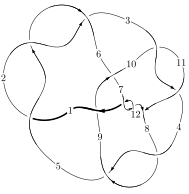
\includegraphics[width=112pt]{../../../GIT/diagram.site/Diagrams/png/2048_12a_1247.png}\\
\ \ \ A knot diagram\footnotemark}&
\allowdisplaybreaks
\textbf{Linearized knot diagam} \\
\cline{2-2}
 &
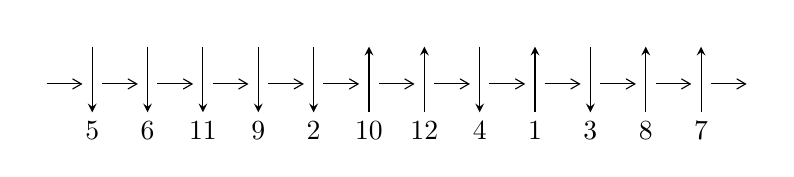
\begin{tikzpicture}[x=20pt, y=17pt]
	% nodes
	\node (C0) at (0, 0) {};
	\node (C1) at (1, 0) {};
	\node (C1U) at (1, +1) {};
	\node (C1D) at (1, -1) {5};

	\node (C2) at (2, 0) {};
	\node (C2U) at (2, +1) {};
	\node (C2D) at (2, -1) {6};

	\node (C3) at (3, 0) {};
	\node (C3U) at (3, +1) {};
	\node (C3D) at (3, -1) {11};

	\node (C4) at (4, 0) {};
	\node (C4U) at (4, +1) {};
	\node (C4D) at (4, -1) {9};

	\node (C5) at (5, 0) {};
	\node (C5U) at (5, +1) {};
	\node (C5D) at (5, -1) {2};

	\node (C6) at (6, 0) {};
	\node (C6U) at (6, +1) {};
	\node (C6D) at (6, -1) {10};

	\node (C7) at (7, 0) {};
	\node (C7U) at (7, +1) {};
	\node (C7D) at (7, -1) {12};

	\node (C8) at (8, 0) {};
	\node (C8U) at (8, +1) {};
	\node (C8D) at (8, -1) {4};

	\node (C9) at (9, 0) {};
	\node (C9U) at (9, +1) {};
	\node (C9D) at (9, -1) {1};

	\node (C10) at (10, 0) {};
	\node (C10U) at (10, +1) {};
	\node (C10D) at (10, -1) {3};

	\node (C11) at (11, 0) {};
	\node (C11U) at (11, +1) {};
	\node (C11D) at (11, -1) {8};

	\node (C12) at (12, 0) {};
	\node (C12U) at (12, +1) {};
	\node (C12D) at (12, -1) {7};
	\node (C13) at (13, 0) {};

	% arrows
	\draw[->,>={angle 60}]
	(C0) edge (C1) (C1) edge (C2) (C2) edge (C3) (C3) edge (C4) (C4) edge (C5) (C5) edge (C6) (C6) edge (C7) (C7) edge (C8) (C8) edge (C9) (C9) edge (C10) (C10) edge (C11) (C11) edge (C12) (C12) edge (C13) ;	\draw[->,>=stealth]
	(C1U) edge (C1D) (C2U) edge (C2D) (C3U) edge (C3D) (C4U) edge (C4D) (C5U) edge (C5D) (C6D) edge (C6U) (C7D) edge (C7U) (C8U) edge (C8D) (C9D) edge (C9U) (C10U) edge (C10D) (C11D) edge (C11U) (C12D) edge (C12U) ;
	\end{tikzpicture} \\
\hhline{~~} \\& 
\textbf{Solving Sequence} \\ \cline{2-2} 
 &
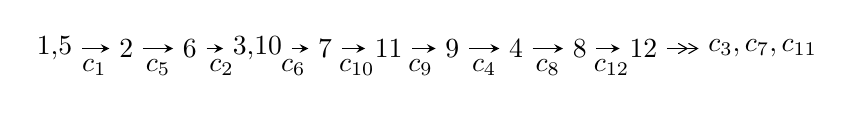
\begin{tikzpicture}[x=23pt, y=7pt]
	% node
	\node (A0) at (-1/8, 0) {1,5};
	\node (A1) at (1, 0) {2};
	\node (A2) at (2, 0) {6};
	\node (A3) at (49/16, 0) {3,10};
	\node (A4) at (33/8, 0) {7};
	\node (A5) at (41/8, 0) {11};
	\node (A6) at (49/8, 0) {9};
	\node (A7) at (57/8, 0) {4};
	\node (A8) at (65/8, 0) {8};
	\node (A9) at (73/8, 0) {12};
	\node (C1) at (1/2, -1) {$c_{1}$};
	\node (C2) at (3/2, -1) {$c_{5}$};
	\node (C3) at (5/2, -1) {$c_{2}$};
	\node (C4) at (29/8, -1) {$c_{6}$};
	\node (C5) at (37/8, -1) {$c_{10}$};
	\node (C6) at (45/8, -1) {$c_{9}$};
	\node (C7) at (53/8, -1) {$c_{4}$};
	\node (C8) at (61/8, -1) {$c_{8}$};
	\node (C9) at (69/8, -1) {$c_{12}$};
	\node (A10) at (11, 0) {$c_{3},c_{7},c_{11}$};

	% edge
	\draw[->,>=stealth]	
	(A0) edge (A1) (A1) edge (A2) (A2) edge (A3) (A3) edge (A4) (A4) edge (A5) (A5) edge (A6) (A6) edge (A7) (A7) edge (A8) (A8) edge (A9) ;
	\draw[->>,>={angle 60}]	
	(A9) edge (A10);
\end{tikzpicture} \\ 

\end{tabular} \\

\footnotetext{
The image of knot diagram is generated by the software ``\textbf{Draw programme}" developed by Andrew Bartholomew(\url{http://www.layer8.co.uk/maths/draw/index.htm\#Running-draw}), where we modified some parts for our purpose(\url{https://github.com/CATsTAILs/LinksPainter}).
}\phantom \\ \newline 
\centering \textbf{Ideals for irreducible components\footnotemark of $X_{\text{par}}$} 
 
\begin{align*}
I^u_{1}&=\langle 
-1931 u^{31}+20740 u^{30}+\cdots+8 b-23592,\;-7773 u^{31}+82554 u^{30}+\cdots+16 a-89232,\\
\phantom{I^u_{1}}&\phantom{= \langle  }u^{32}-12 u^{31}+\cdots-48 u-16\rangle \\
I^u_{2}&=\langle 
-1.02625\times10^{22} a^{7} u^{5}+8.99106\times10^{21} a^{6} u^{5}+\cdots-4.39399\times10^{21} a+3.98524\times10^{22},\\
\phantom{I^u_{2}}&\phantom{= \langle  }- a^7 u^5+8 a^6 u^5+\cdots-489 a+821,\;u^6+u^5-3 u^4-2 u^3+2 u^2- u-1\rangle \\
I^u_{3}&=\langle 
u^{21}+2 u^{20}+\cdots+b+u,\;4 u^{21}+8 u^{20}+\cdots+a+5,\;u^{22}+3 u^{21}+\cdots+3 u+1\rangle \\
\\
\end{align*}
\raggedright * 3 irreducible components of $\dim_{\mathbb{C}}=0$, with total 102 representations.\\
\footnotetext{All coefficients of polynomials are rational numbers. But the coefficients are sometimes approximated in decimal forms when there is not enough margin.}
\newpage
\renewcommand{\arraystretch}{1}
\centering \section*{I. $I^u_{1}= \langle -1931 u^{31}+20740 u^{30}+\cdots+8 b-23592,\;-7773 u^{31}+82554 u^{30}+\cdots+16 a-89232,\;u^{32}-12 u^{31}+\cdots-48 u-16 \rangle$}
\flushleft \textbf{(i) Arc colorings}\\
\begin{tabular}{m{7pt} m{180pt} m{7pt} m{180pt} }
\flushright $a_{1}=$&$\begin{pmatrix}1\\0\end{pmatrix}$ \\
\flushright $a_{5}=$&$\begin{pmatrix}0\\u\end{pmatrix}$ \\
\flushright $a_{2}=$&$\begin{pmatrix}1\\u^2\end{pmatrix}$ \\
\flushright $a_{6}=$&$\begin{pmatrix}- u\\- u^3+u\end{pmatrix}$ \\
\flushright $a_{3}=$&$\begin{pmatrix}- u^2+1\\- u^4+2 u^2\end{pmatrix}$ \\
\flushright $a_{10}=$&$\begin{pmatrix}\frac{7773}{16} u^{31}-\frac{41277}{8} u^{30}+\cdots+\frac{41415}{2} u+5577\\\frac{1931}{8} u^{31}-\frac{5185}{2} u^{30}+\cdots+11043 u+2949\end{pmatrix}$ \\
\flushright $a_{7}=$&$\begin{pmatrix}\frac{107}{2} u^{31}-546 u^{30}+\cdots+\frac{3227}{2} u+\frac{921}{2}\\\frac{143}{2} u^{31}-740 u^{30}+\cdots+\frac{4873}{2} u+680\end{pmatrix}$ \\
\flushright $a_{11}=$&$\begin{pmatrix}\frac{247}{16} u^{31}-\frac{1881}{8} u^{30}+\cdots+\frac{5429}{2} u+656\\-\frac{181}{8} u^{31}+\frac{345}{2} u^{30}+\cdots+1311 u+261\end{pmatrix}$ \\
\flushright $a_{9}=$&$\begin{pmatrix}\frac{3911}{16} u^{31}-\frac{20537}{8} u^{30}+\cdots+\frac{19329}{2} u+2628\\\frac{1931}{8} u^{31}-\frac{5185}{2} u^{30}+\cdots+11043 u+2949\end{pmatrix}$ \\
\flushright $a_{4}=$&$\begin{pmatrix}\frac{43}{2} u^{31}-\frac{441}{2} u^{30}+\cdots+660 u+\frac{377}{2}\\22 u^{31}-240 u^{30}+\cdots+\frac{2169}{2} u+288\end{pmatrix}$ \\
\flushright $a_{8}=$&$\begin{pmatrix}\frac{2271}{8} u^{31}-\frac{24371}{8} u^{30}+\cdots+13172 u+\frac{7009}{2}\\-\frac{1689}{8} u^{31}+\frac{8795}{4} u^{30}+\cdots-\frac{14811}{2} u-2064\end{pmatrix}$ \\
\flushright $a_{12}=$&$\begin{pmatrix}566 u^{31}-\frac{23745}{4} u^{30}+\cdots+\frac{86833}{4} u+5945\\355 u^{31}-\frac{14985}{4} u^{30}+\cdots+14324 u+3892\end{pmatrix}$\\&\end{tabular}
\flushleft \textbf{(ii) Obstruction class $= -1$}\\~\\
\flushleft \textbf{(iii) Cusp Shapes $= \frac{4311}{2} u^{31}-22730 u^{30}+\cdots+87134 u+23654$}\\~\\
\newpage\renewcommand{\arraystretch}{1}
\flushleft \textbf{(iv) u-Polynomials at the component}\newline \\
\begin{tabular}{m{50pt}|m{274pt}}
Crossings & \hspace{64pt}u-Polynomials at each crossing \\
\hline $$\begin{aligned}c_{1},c_{2},c_{5}\end{aligned}$$&$\begin{aligned}
&u^{32}+12 u^{31}+\cdots+48 u-16
\end{aligned}$\\
\hline $$\begin{aligned}c_{3},c_{4},c_{8}\\c_{10}\end{aligned}$$&$\begin{aligned}
&u^{32}- u^{31}+\cdots+u^2+1
\end{aligned}$\\
\hline $$\begin{aligned}c_{6},c_{9}\end{aligned}$$&$\begin{aligned}
&u^{32}+u^{31}+\cdots-17 u-1
\end{aligned}$\\
\hline $$\begin{aligned}c_{7},c_{11},c_{12}\end{aligned}$$&$\begin{aligned}
&u^{32}-14 u^{31}+\cdots+736 u-64
\end{aligned}$\\
\hline
\end{tabular}\\~\\
\newpage\renewcommand{\arraystretch}{1}
\flushleft \textbf{(v) Riley Polynomials at the component}\newline \\
\begin{tabular}{m{50pt}|m{274pt}}
Crossings & \hspace{64pt}Riley Polynomials at each crossing \\
\hline $$\begin{aligned}c_{1},c_{2},c_{5}\end{aligned}$$&$\begin{aligned}
&y^{32}-32 y^{31}+\cdots-1408 y+256
\end{aligned}$\\
\hline $$\begin{aligned}c_{3},c_{4},c_{8}\\c_{10}\end{aligned}$$&$\begin{aligned}
&y^{32}-35 y^{31}+\cdots+2 y+1
\end{aligned}$\\
\hline $$\begin{aligned}c_{6},c_{9}\end{aligned}$$&$\begin{aligned}
&y^{32}+25 y^{31}+\cdots-121 y+1
\end{aligned}$\\
\hline $$\begin{aligned}c_{7},c_{11},c_{12}\end{aligned}$$&$\begin{aligned}
&y^{32}+30 y^{31}+\cdots-46080 y+4096
\end{aligned}$\\
\hline
\end{tabular}\\~\\
\newpage\flushleft \textbf{(vi) Complex Volumes and Cusp Shapes}
$$\begin{array}{c|c|c}  
\text{Solutions to }I^u_{1}& \I (\text{vol} + \sqrt{-1}CS) & \text{Cusp shape}\\
 \hline 
\begin{aligned}
u &= -0.680828 + 0.815159 I \\
a &= \phantom{-}0.589852 - 0.500904 I \\
b &= -0.68125 - 1.37591 I\end{aligned}
 & -15.1501 + 11.2353 I & -10.12137 - 6.63149 I \\ \hline\begin{aligned}
u &= -0.680828 - 0.815159 I \\
a &= \phantom{-}0.589852 + 0.500904 I \\
b &= -0.68125 + 1.37591 I\end{aligned}
 & -15.1501 - 11.2353 I & -10.12137 + 6.63149 I \\ \hline\begin{aligned}
u &= -0.494831 + 0.951026 I \\
a &= -0.617680 - 0.176687 I \\
b &= -0.232561 + 1.197900 I\end{aligned}
 & -14.5005 - 5.4219 I & -10.91537 + 2.28879 I \\ \hline\begin{aligned}
u &= -0.494831 - 0.951026 I \\
a &= -0.617680 + 0.176687 I \\
b &= -0.232561 - 1.197900 I\end{aligned}
 & -14.5005 + 5.4219 I & -10.91537 - 2.28879 I \\ \hline\begin{aligned}
u &= -1.14307\phantom{ +0.000000I} \\
a &= -0.439539\phantom{ +0.000000I} \\
b &= -1.07672\phantom{ +0.000000I}\end{aligned}
 & -1.32792\phantom{ +0.000000I} & -8.36980\phantom{ +0.000000I} \\ \hline\begin{aligned}
u &= -0.713057 + 0.906916 I \\
a &= -0.473999 + 0.283951 I \\
b &= \phantom{-}0.435641 + 1.156230 I\end{aligned}
 & -7.22904 + 6.56235 I & \phantom{-0.000000 } 0 \\ \hline\begin{aligned}
u &= -0.713057 - 0.906916 I \\
a &= -0.473999 - 0.283951 I \\
b &= \phantom{-}0.435641 - 1.156230 I\end{aligned}
 & -7.22904 - 6.56235 I & \phantom{-0.000000 } 0 \\ \hline\begin{aligned}
u &= -0.615956 + 1.004530 I \\
a &= \phantom{-}0.488535 - 0.045297 I \\
b &= -0.108266 - 1.094690 I\end{aligned}
 & -6.84872 - 0.16660 I & \phantom{-0.000000 } 0 \\ \hline\begin{aligned}
u &= -0.615956 - 1.004530 I \\
a &= \phantom{-}0.488535 + 0.045297 I \\
b &= -0.108266 + 1.094690 I\end{aligned}
 & -6.84872 + 0.16660 I & \phantom{-0.000000 } 0 \\ \hline\begin{aligned}
u &= \phantom{-}1.157610 + 0.416068 I \\
a &= \phantom{-}0.506893 - 0.188759 I \\
b &= \phantom{-}0.108022 + 0.275619 I\end{aligned}
 & -4.34328 - 2.34802 I & \phantom{-0.000000 } 0\\
 \hline 
 \end{array}$$\newpage$$\begin{array}{c|c|c}  
\text{Solutions to }I^u_{1}& \I (\text{vol} + \sqrt{-1}CS) & \text{Cusp shape}\\
 \hline 
\begin{aligned}
u &= \phantom{-}1.157610 - 0.416068 I \\
a &= \phantom{-}0.506893 + 0.188759 I \\
b &= \phantom{-}0.108022 - 0.275619 I\end{aligned}
 & -4.34328 + 2.34802 I & \phantom{-0.000000 } 0 \\ \hline\begin{aligned}
u &= -1.232110 + 0.231185 I \\
a &= \phantom{-}0.300965 + 0.165464 I \\
b &= \phantom{-}0.944141 + 0.205181 I\end{aligned}
 & -4.97841 + 4.31582 I & \phantom{-0.000000 } 0 \\ \hline\begin{aligned}
u &= -1.232110 - 0.231185 I \\
a &= \phantom{-}0.300965 - 0.165464 I \\
b &= \phantom{-}0.944141 - 0.205181 I\end{aligned}
 & -4.97841 - 4.31582 I & \phantom{-0.000000 } 0 \\ \hline\begin{aligned}
u &= \phantom{-}0.739575\phantom{ +0.000000I} \\
a &= -0.445134\phantom{ +0.000000I} \\
b &= \phantom{-}0.0857344\phantom{ +0.000000I}\end{aligned}
 & -0.987038\phantom{ +0.000000I} & -12.9270\phantom{ +0.000000I} \\ \hline\begin{aligned}
u &= \phantom{-}0.057187 + 0.603926 I \\
a &= -0.204724 + 0.701064 I \\
b &= \phantom{-}0.460672 - 0.183999 I\end{aligned}
 & -1.25850 - 1.44721 I & -2.35502 + 5.22658 I \\ \hline\begin{aligned}
u &= \phantom{-}0.057187 - 0.603926 I \\
a &= -0.204724 - 0.701064 I \\
b &= \phantom{-}0.460672 + 0.183999 I\end{aligned}
 & -1.25850 + 1.44721 I & -2.35502 - 5.22658 I \\ \hline\begin{aligned}
u &= \phantom{-}1.45355 + 0.03396 I \\
a &= -0.23567 + 1.66598 I \\
b &= -0.262994 + 1.081130 I\end{aligned}
 & -4.57485 - 1.68293 I & \phantom{-0.000000 } 0 \\ \hline\begin{aligned}
u &= \phantom{-}1.45355 - 0.03396 I \\
a &= -0.23567 - 1.66598 I \\
b &= -0.262994 - 1.081130 I\end{aligned}
 & -4.57485 + 1.68293 I & \phantom{-0.000000 } 0 \\ \hline\begin{aligned}
u &= \phantom{-}1.50382 + 0.05578 I \\
a &= \phantom{-}0.50318 - 1.98250 I \\
b &= \phantom{-}0.60170 - 1.43953 I\end{aligned}
 & -10.29120 - 4.14932 I & \phantom{-0.000000 } 0 \\ \hline\begin{aligned}
u &= \phantom{-}1.50382 - 0.05578 I \\
a &= \phantom{-}0.50318 + 1.98250 I \\
b &= \phantom{-}0.60170 + 1.43953 I\end{aligned}
 & -10.29120 + 4.14932 I & \phantom{-0.000000 } 0\\
 \hline 
 \end{array}$$\newpage$$\begin{array}{c|c|c}  
\text{Solutions to }I^u_{1}& \I (\text{vol} + \sqrt{-1}CS) & \text{Cusp shape}\\
 \hline 
\begin{aligned}
u &= -0.456157 + 0.188264 I \\
a &= \phantom{-}0.30670 + 1.62184 I \\
b &= \phantom{-}0.776747 + 0.909381 I\end{aligned}
 & -3.74818 + 3.21761 I & \phantom{-}2.70792 - 3.34583 I \\ \hline\begin{aligned}
u &= -0.456157 - 0.188264 I \\
a &= \phantom{-}0.30670 - 1.62184 I \\
b &= \phantom{-}0.776747 - 0.909381 I\end{aligned}
 & -3.74818 - 3.21761 I & \phantom{-}2.70792 + 3.34583 I \\ \hline\begin{aligned}
u &= -0.247450 + 0.286515 I \\
a &= \phantom{-}0.10986 - 1.41840 I \\
b &= -0.582621 - 0.368449 I\end{aligned}
 & \phantom{-}0.987106 + 0.748744 I & \phantom{-}5.19413 - 3.21537 I \\ \hline\begin{aligned}
u &= -0.247450 - 0.286515 I \\
a &= \phantom{-}0.10986 + 1.41840 I \\
b &= -0.582621 + 0.368449 I\end{aligned}
 & \phantom{-}0.987106 - 0.748744 I & \phantom{-}5.19413 + 3.21537 I \\ \hline\begin{aligned}
u &= \phantom{-}1.60347 + 0.26376 I \\
a &= \phantom{-}0.08484 + 1.83824 I \\
b &= -0.99385 + 1.70026 I\end{aligned}
 & \phantom{-}16.7864 - 15.2459 I & \phantom{-0.000000 } 0 \\ \hline\begin{aligned}
u &= \phantom{-}1.60347 - 0.26376 I \\
a &= \phantom{-}0.08484 - 1.83824 I \\
b &= -0.99385 - 1.70026 I\end{aligned}
 & \phantom{-}16.7864 + 15.2459 I & \phantom{-0.000000 } 0 \\ \hline\begin{aligned}
u &= \phantom{-}1.60023 + 0.36433 I \\
a &= -0.567147 - 0.962796 I \\
b &= \phantom{-}0.302404 - 1.251650 I\end{aligned}
 & \phantom{-}18.1780 + 0.4768 I & \phantom{-0.000000 } 0 \\ \hline\begin{aligned}
u &= \phantom{-}1.60023 - 0.36433 I \\
a &= -0.567147 + 0.962796 I \\
b &= \phantom{-}0.302404 + 1.251650 I\end{aligned}
 & \phantom{-}18.1780 - 0.4768 I & \phantom{-0.000000 } 0 \\ \hline\begin{aligned}
u &= \phantom{-}1.62632 + 0.27751 I \\
a &= -0.07773 - 1.52430 I \\
b &= \phantom{-}0.87969 - 1.48385 I\end{aligned}
 & -14.9769 - 10.9327 I & \phantom{-0.000000 } 0 \\ \hline\begin{aligned}
u &= \phantom{-}1.62632 - 0.27751 I \\
a &= -0.07773 + 1.52430 I \\
b &= \phantom{-}0.87969 + 1.48385 I\end{aligned}
 & -14.9769 + 10.9327 I & \phantom{-0.000000 } 0\\
 \hline 
 \end{array}$$\newpage$$\begin{array}{c|c|c}  
\text{Solutions to }I^u_{1}& \I (\text{vol} + \sqrt{-1}CS) & \text{Cusp shape}\\
 \hline 
\begin{aligned}
u &= \phantom{-}1.63995 + 0.31827 I \\
a &= \phantom{-}0.228456 + 1.197060 I \\
b &= -0.65199 + 1.30081 I\end{aligned}
 & -14.3366 - 4.7680 I & \phantom{-0.000000 } 0 \\ \hline\begin{aligned}
u &= \phantom{-}1.63995 - 0.31827 I \\
a &= \phantom{-}0.228456 - 1.197060 I \\
b &= -0.65199 - 1.30081 I\end{aligned}
 & -14.3366 + 4.7680 I & \phantom{-0.000000 } 0\\
 \hline 
 \end{array}$$\newpage\newpage\renewcommand{\arraystretch}{1}
\centering \section*{II. $I^u_{2}= \langle -1.03\times10^{22} a^{7} u^{5}+8.99\times10^{21} a^{6} u^{5}+\cdots-4.39\times10^{21} a+3.99\times10^{22},\;- a^7 u^5+8 a^6 u^5+\cdots-489 a+821,\;u^6+u^5-3 u^4-2 u^3+2 u^2- u-1 \rangle$}
\flushleft \textbf{(i) Arc colorings}\\
\begin{tabular}{m{7pt} m{180pt} m{7pt} m{180pt} }
\flushright $a_{1}=$&$\begin{pmatrix}1\\0\end{pmatrix}$ \\
\flushright $a_{5}=$&$\begin{pmatrix}0\\u\end{pmatrix}$ \\
\flushright $a_{2}=$&$\begin{pmatrix}1\\u^2\end{pmatrix}$ \\
\flushright $a_{6}=$&$\begin{pmatrix}- u\\- u^3+u\end{pmatrix}$ \\
\flushright $a_{3}=$&$\begin{pmatrix}- u^2+1\\- u^4+2 u^2\end{pmatrix}$ \\
\flushright $a_{10}=$&$\begin{pmatrix}a\\0.493774 a^{7} u^{5}-0.432600 a^{6} u^{5}+\cdots+0.211415 a-1.91748\end{pmatrix}$ \\
\flushright $a_{7}=$&$\begin{pmatrix}-0.0990366 a^{7} u^{5}+0.0845549 a^{6} u^{5}+\cdots+0.244699 a+0.622156\\0.550411 a^{7} u^{5}-1.43426 a^{6} u^{5}+\cdots-0.965495 a-1.46874\end{pmatrix}$ \\
\flushright $a_{11}=$&$\begin{pmatrix}-1.24509 a^{7} u^{5}+1.54783 a^{6} u^{5}+\cdots+0.631576 a+0.985297\\0.939975 a^{7} u^{5}-1.15258 a^{6} u^{5}+\cdots-0.412776 a-2.64976\end{pmatrix}$ \\
\flushright $a_{9}=$&$\begin{pmatrix}-0.493774 a^{7} u^{5}+0.432600 a^{6} u^{5}+\cdots+0.788585 a+1.91748\\0.493774 a^{7} u^{5}-0.432600 a^{6} u^{5}+\cdots+0.211415 a-1.91748\end{pmatrix}$ \\
\flushright $a_{4}=$&$\begin{pmatrix}1.15029 a^{7} u^{5}-1.79608 a^{6} u^{5}+\cdots-1.16871 a-4.70289\\-1.05125 a^{7} u^{5}+1.71153 a^{6} u^{5}+\cdots+0.924014 a+4.08073\end{pmatrix}$ \\
\flushright $a_{8}=$&$\begin{pmatrix}0.634934 a^{7} u^{5}-1.65705 a^{6} u^{5}+\cdots-2.68099 a-1.05272\\-0.970106 a^{7} u^{5}+1.96530 a^{6} u^{5}+\cdots+1.88294 a+3.88034\end{pmatrix}$ \\
\flushright $a_{12}=$&$\begin{pmatrix}-0.590593 a^{7} u^{5}+1.21867 a^{6} u^{5}+\cdots+0.288049 a+1.83640\\0.520280 a^{7} u^{5}-0.621535 a^{6} u^{5}+\cdots+0.504665 a-1.23816\end{pmatrix}$\\&\end{tabular}
\flushleft \textbf{(ii) Obstruction class $= -1$}\\~\\
\flushleft \textbf{(iii) Cusp Shapes $= \frac{32386428834844106415168}{20783768619782088516773} a^7 u^5+\frac{23417790588849644990728}{20783768619782088516773} a^6 u^5+\cdots+\frac{45950322676565104630412}{20783768619782088516773} a-\frac{306021993643431809155814}{20783768619782088516773}$}\\~\\
\newpage\renewcommand{\arraystretch}{1}
\flushleft \textbf{(iv) u-Polynomials at the component}\newline \\
\begin{tabular}{m{50pt}|m{274pt}}
Crossings & \hspace{64pt}u-Polynomials at each crossing \\
\hline $$\begin{aligned}c_{1},c_{2},c_{5}\end{aligned}$$&$\begin{aligned}
&(u^6- u^5-3 u^4+2 u^3+2 u^2+u-1)^8
\end{aligned}$\\
\hline $$\begin{aligned}c_{3},c_{4},c_{8}\\c_{10}\end{aligned}$$&$\begin{aligned}
&u^{48}+u^{47}+\cdots-1444 u+479
\end{aligned}$\\
\hline $$\begin{aligned}c_{6},c_{9}\end{aligned}$$&$\begin{aligned}
&u^{48}-7 u^{47}+\cdots-40272 u+71579
\end{aligned}$\\
\hline $$\begin{aligned}c_{7},c_{11},c_{12}\end{aligned}$$&$\begin{aligned}
&(u^4+u^3+3 u^2+2 u+1)^{12}
\end{aligned}$\\
\hline
\end{tabular}\\~\\
\newpage\renewcommand{\arraystretch}{1}
\flushleft \textbf{(v) Riley Polynomials at the component}\newline \\
\begin{tabular}{m{50pt}|m{274pt}}
Crossings & \hspace{64pt}Riley Polynomials at each crossing \\
\hline $$\begin{aligned}c_{1},c_{2},c_{5}\end{aligned}$$&$\begin{aligned}
&(y^6-7 y^5+17 y^4-16 y^3+6 y^2-5 y+1)^8
\end{aligned}$\\
\hline $$\begin{aligned}c_{3},c_{4},c_{8}\\c_{10}\end{aligned}$$&$\begin{aligned}
&y^{48}-49 y^{47}+\cdots+10146608 y+229441
\end{aligned}$\\
\hline $$\begin{aligned}c_{6},c_{9}\end{aligned}$$&$\begin{aligned}
&y^{48}+23 y^{47}+\cdots+117241967100 y+5123553241
\end{aligned}$\\
\hline $$\begin{aligned}c_{7},c_{11},c_{12}\end{aligned}$$&$\begin{aligned}
&(y^4+5 y^3+7 y^2+2 y+1)^{12}
\end{aligned}$\\
\hline
\end{tabular}\\~\\
\newpage\flushleft \textbf{(vi) Complex Volumes and Cusp Shapes}
$$\begin{array}{c|c|c}  
\text{Solutions to }I^u_{2}& \I (\text{vol} + \sqrt{-1}CS) & \text{Cusp shape}\\
 \hline 
\begin{aligned}
u &= \phantom{-}0.493180 + 0.575288 I \\
a &= -0.900819 + 0.089225 I \\
b &= \phantom{-}0.127208 - 0.784719 I\end{aligned}
 & -1.76355 - 0.55731 I & -4.74899 - 1.22396 I \\ \hline\begin{aligned}
u &= \phantom{-}0.493180 + 0.575288 I \\
a &= -0.488061 - 1.039120 I \\
b &= \phantom{-}0.459656 - 0.638436 I\end{aligned}
 & -1.76355 - 3.38752 I & -4.74899 + 8.59352 I \\ \hline\begin{aligned}
u &= \phantom{-}0.493180 + 0.575288 I \\
a &= -0.630925 - 0.290654 I \\
b &= \phantom{-}0.70939 - 1.58712 I\end{aligned}
 & -8.76530 - 5.13637 I & -8.40246 + 6.24958 I \\ \hline\begin{aligned}
u &= \phantom{-}0.493180 + 0.575288 I \\
a &= \phantom{-}0.601944 + 0.215661 I \\
b &= -0.532273 + 1.115900 I\end{aligned}
 & -1.76355 - 3.38752 I & -4.74899 + 8.59352 I \\ \hline\begin{aligned}
u &= \phantom{-}0.493180 + 0.575288 I \\
a &= \phantom{-}1.55616 - 0.32740 I \\
b &= \phantom{-}0.215809 + 1.064350 I\end{aligned}
 & -8.76530 + 1.19155 I & -8.40246 + 1.11998 I \\ \hline\begin{aligned}
u &= \phantom{-}0.493180 + 0.575288 I \\
a &= \phantom{-}0.181370 + 0.327241 I \\
b &= \phantom{-}0.293994 + 0.548435 I\end{aligned}
 & -1.76355 - 0.55731 I & -4.74899 - 1.22396 I \\ \hline\begin{aligned}
u &= \phantom{-}0.493180 + 0.575288 I \\
a &= -0.295940 + 0.035805 I \\
b &= -0.950173 - 0.904845 I\end{aligned}
 & -8.76530 + 1.19155 I & -8.40246 + 1.11998 I \\ \hline\begin{aligned}
u &= \phantom{-}0.493180 + 0.575288 I \\
a &= \phantom{-}0.83692 + 1.56767 I \\
b &= -0.819030 + 0.843679 I\end{aligned}
 & -8.76530 - 5.13637 I & -8.40246 + 6.24958 I \\ \hline\begin{aligned}
u &= \phantom{-}0.493180 - 0.575288 I \\
a &= -0.900819 - 0.089225 I \\
b &= \phantom{-}0.127208 + 0.784719 I\end{aligned}
 & -1.76355 + 0.55731 I & -4.74899 + 1.22396 I \\ \hline\begin{aligned}
u &= \phantom{-}0.493180 - 0.575288 I \\
a &= -0.488061 + 1.039120 I \\
b &= \phantom{-}0.459656 + 0.638436 I\end{aligned}
 & -1.76355 + 3.38752 I & -4.74899 - 8.59352 I\\
 \hline 
 \end{array}$$\newpage$$\begin{array}{c|c|c}  
\text{Solutions to }I^u_{2}& \I (\text{vol} + \sqrt{-1}CS) & \text{Cusp shape}\\
 \hline 
\begin{aligned}
u &= \phantom{-}0.493180 - 0.575288 I \\
a &= -0.630925 + 0.290654 I \\
b &= \phantom{-}0.70939 + 1.58712 I\end{aligned}
 & -8.76530 + 5.13637 I & -8.40246 - 6.24958 I \\ \hline\begin{aligned}
u &= \phantom{-}0.493180 - 0.575288 I \\
a &= \phantom{-}0.601944 - 0.215661 I \\
b &= -0.532273 - 1.115900 I\end{aligned}
 & -1.76355 + 3.38752 I & -4.74899 - 8.59352 I \\ \hline\begin{aligned}
u &= \phantom{-}0.493180 - 0.575288 I \\
a &= \phantom{-}1.55616 + 0.32740 I \\
b &= \phantom{-}0.215809 - 1.064350 I\end{aligned}
 & -8.76530 - 1.19155 I & -8.40246 - 1.11998 I \\ \hline\begin{aligned}
u &= \phantom{-}0.493180 - 0.575288 I \\
a &= \phantom{-}0.181370 - 0.327241 I \\
b &= \phantom{-}0.293994 - 0.548435 I\end{aligned}
 & -1.76355 + 0.55731 I & -4.74899 + 1.22396 I \\ \hline\begin{aligned}
u &= \phantom{-}0.493180 - 0.575288 I \\
a &= -0.295940 - 0.035805 I \\
b &= -0.950173 + 0.904845 I\end{aligned}
 & -8.76530 - 1.19155 I & -8.40246 - 1.11998 I \\ \hline\begin{aligned}
u &= \phantom{-}0.493180 - 0.575288 I \\
a &= \phantom{-}0.83692 - 1.56767 I \\
b &= -0.819030 - 0.843679 I\end{aligned}
 & -8.76530 + 5.13637 I & -8.40246 - 6.24958 I \\ \hline\begin{aligned}
u &= -0.483672\phantom{ +0.000000I} \\
a &= \phantom{-}1.243000 + 0.503165 I \\
b &= -1.55666 + 1.20761 I\end{aligned}
 & -12.46440 + 3.16396 I & -17.2435 - 2.5648 I \\ \hline\begin{aligned}
u &= -0.483672\phantom{ +0.000000I} \\
a &= \phantom{-}1.243000 - 0.503165 I \\
b &= -1.55666 - 1.20761 I\end{aligned}
 & -12.46440 - 3.16396 I & -17.2435 + 2.5648 I \\ \hline\begin{aligned}
u &= -0.483672\phantom{ +0.000000I} \\
a &= -1.68596 + 0.76343 I \\
b &= \phantom{-}0.935756 + 0.863246 I\end{aligned}
 & -5.46265 - 1.41510 I & -13.5900 + 4.9087 I \\ \hline\begin{aligned}
u &= -0.483672\phantom{ +0.000000I} \\
a &= -1.68596 - 0.76343 I \\
b &= \phantom{-}0.935756 - 0.863246 I\end{aligned}
 & -5.46265 + 1.41510 I & -13.5900 - 4.9087 I\\
 \hline 
 \end{array}$$\newpage$$\begin{array}{c|c|c}  
\text{Solutions to }I^u_{2}& \I (\text{vol} + \sqrt{-1}CS) & \text{Cusp shape}\\
 \hline 
\begin{aligned}
u &= -0.483672\phantom{ +0.000000I} \\
a &= \phantom{-}2.75014 + 1.41553 I \\
b &= -0.172089 + 0.700395 I\end{aligned}
 & -5.46265 - 1.41510 I & -13.5900 + 4.9087 I \\ \hline\begin{aligned}
u &= -0.483672\phantom{ +0.000000I} \\
a &= \phantom{-}2.75014 - 1.41553 I \\
b &= -0.172089 - 0.700395 I\end{aligned}
 & -5.46265 + 1.41510 I & -13.5900 - 4.9087 I \\ \hline\begin{aligned}
u &= -0.483672\phantom{ +0.000000I} \\
a &= -3.81963 + 2.25339 I \\
b &= -0.292353 + 0.770523 I\end{aligned}
 & -12.46440 + 3.16396 I & -17.2435 - 2.5648 I \\ \hline\begin{aligned}
u &= -0.483672\phantom{ +0.000000I} \\
a &= -3.81963 - 2.25339 I \\
b &= -0.292353 - 0.770523 I\end{aligned}
 & -12.46440 - 3.16396 I & -17.2435 + 2.5648 I \\ \hline\begin{aligned}
u &= -1.52087 + 0.16310 I \\
a &= \phantom{-}0.782884 - 1.127760 I \\
b &= -0.343085 - 1.002600 I\end{aligned}
 & -15.4211 + 1.4282 I & -12.40788 - 0.64002 I \\ \hline\begin{aligned}
u &= -1.52087 + 0.16310 I \\
a &= -0.200569 + 1.374100 I \\
b &= \phantom{-}0.675225 + 1.150860 I\end{aligned}
 & -8.41938 + 3.17702 I & -8.75440 + 1.70392 I \\ \hline\begin{aligned}
u &= -1.52087 + 0.16310 I \\
a &= \phantom{-}0.439631 - 1.327350 I \\
b &= \phantom{-}0.265769 - 1.130460 I\end{aligned}
 & -8.41938 + 3.17702 I & -8.75440 + 1.70392 I \\ \hline\begin{aligned}
u &= -1.52087 + 0.16310 I \\
a &= -1.15986 + 1.16720 I \\
b &= -1.06617 + 1.40127 I\end{aligned}
 & -15.4211 + 1.4282 I & -12.40788 - 0.64002 I \\ \hline\begin{aligned}
u &= -1.52087 + 0.16310 I \\
a &= -0.04775 + 1.70162 I \\
b &= \phantom{-}0.327173 + 1.006110 I\end{aligned}
 & -8.41938 + 6.00723 I & -8.75440 - 8.11356 I \\ \hline\begin{aligned}
u &= -1.52087 + 0.16310 I \\
a &= -0.06236 - 1.91890 I \\
b &= -0.88964 - 1.76077 I\end{aligned}
 & -8.41938 + 6.00723 I & -8.75440 - 8.11356 I\\
 \hline 
 \end{array}$$\newpage$$\begin{array}{c|c|c}  
\text{Solutions to }I^u_{2}& \I (\text{vol} + \sqrt{-1}CS) & \text{Cusp shape}\\
 \hline 
\begin{aligned}
u &= -1.52087 + 0.16310 I \\
a &= -0.07791 - 2.08226 I \\
b &= -0.593633 - 1.010750 I\end{aligned}
 & -15.4211 + 7.7561 I & -12.40788 - 5.76962 I \\ \hline\begin{aligned}
u &= -1.52087 + 0.16310 I \\
a &= \phantom{-}0.14267 + 2.45572 I \\
b &= \phantom{-}1.08638 + 2.38993 I\end{aligned}
 & -15.4211 + 7.7561 I & -12.40788 - 5.76962 I \\ \hline\begin{aligned}
u &= -1.52087 - 0.16310 I \\
a &= \phantom{-}0.782884 + 1.127760 I \\
b &= -0.343085 + 1.002600 I\end{aligned}
 & -15.4211 - 1.4282 I & -12.40788 + 0.64002 I \\ \hline\begin{aligned}
u &= -1.52087 - 0.16310 I \\
a &= -0.200569 - 1.374100 I \\
b &= \phantom{-}0.675225 - 1.150860 I\end{aligned}
 & -8.41938 - 3.17702 I & -8.75440 - 1.70392 I \\ \hline\begin{aligned}
u &= -1.52087 - 0.16310 I \\
a &= \phantom{-}0.439631 + 1.327350 I \\
b &= \phantom{-}0.265769 + 1.130460 I\end{aligned}
 & -8.41938 - 3.17702 I & -8.75440 - 1.70392 I \\ \hline\begin{aligned}
u &= -1.52087 - 0.16310 I \\
a &= -1.15986 - 1.16720 I \\
b &= -1.06617 - 1.40127 I\end{aligned}
 & -15.4211 - 1.4282 I & -12.40788 + 0.64002 I \\ \hline\begin{aligned}
u &= -1.52087 - 0.16310 I \\
a &= -0.04775 - 1.70162 I \\
b &= \phantom{-}0.327173 - 1.006110 I\end{aligned}
 & -8.41938 - 6.00723 I & -8.75440 + 8.11356 I \\ \hline\begin{aligned}
u &= -1.52087 - 0.16310 I \\
a &= -0.06236 + 1.91890 I \\
b &= -0.88964 + 1.76077 I\end{aligned}
 & -8.41938 - 6.00723 I & -8.75440 + 8.11356 I \\ \hline\begin{aligned}
u &= -1.52087 - 0.16310 I \\
a &= -0.07791 + 2.08226 I \\
b &= -0.593633 + 1.010750 I\end{aligned}
 & -15.4211 - 7.7561 I & -12.40788 + 5.76962 I \\ \hline\begin{aligned}
u &= -1.52087 - 0.16310 I \\
a &= \phantom{-}0.14267 - 2.45572 I \\
b &= \phantom{-}1.08638 - 2.38993 I\end{aligned}
 & -15.4211 - 7.7561 I & -12.40788 + 5.76962 I\\
 \hline 
 \end{array}$$\newpage$$\begin{array}{c|c|c}  
\text{Solutions to }I^u_{2}& \I (\text{vol} + \sqrt{-1}CS) & \text{Cusp shape}\\
 \hline 
\begin{aligned}
u &= \phantom{-}1.53904\phantom{ +0.000000I} \\
a &= \phantom{-}0.244560 + 1.155160 I \\
b &= -0.847287 + 0.822406 I\end{aligned}
 & -12.38390 - 1.41510 I & -12.44276 + 4.90874 I \\ \hline\begin{aligned}
u &= \phantom{-}1.53904\phantom{ +0.000000I} \\
a &= \phantom{-}0.244560 - 1.155160 I \\
b &= -0.847287 - 0.822406 I\end{aligned}
 & -12.38390 + 1.41510 I & -12.44276 - 4.90874 I \\ \hline\begin{aligned}
u &= \phantom{-}1.53904\phantom{ +0.000000I} \\
a &= \phantom{-}0.92692 + 1.24349 I \\
b &= \phantom{-}1.81916 + 1.16754 I\end{aligned}
 & -12.38390 - 1.41510 I & -12.44276 + 4.90874 I \\ \hline\begin{aligned}
u &= \phantom{-}1.53904\phantom{ +0.000000I} \\
a &= \phantom{-}0.92692 - 1.24349 I \\
b &= \phantom{-}1.81916 - 1.16754 I\end{aligned}
 & -12.38390 + 1.41510 I & -12.44276 - 4.90874 I \\ \hline\begin{aligned}
u &= \phantom{-}1.53904\phantom{ +0.000000I} \\
a &= -1.03576 + 1.39658 I \\
b &= \phantom{-}0.317947 + 0.787184 I\end{aligned}
 & -19.3856 + 3.1640 I & -16.0962 - 2.5648 I \\ \hline\begin{aligned}
u &= \phantom{-}1.53904\phantom{ +0.000000I} \\
a &= -1.03576 - 1.39658 I \\
b &= \phantom{-}0.317947 - 0.787184 I\end{aligned}
 & -19.3856 - 3.1640 I & -16.0962 + 2.5648 I \\ \hline\begin{aligned}
u &= \phantom{-}1.53904\phantom{ +0.000000I} \\
a &= -1.80066 + 1.63792 I \\
b &= -2.67107 + 1.73026 I\end{aligned}
 & -19.3856 + 3.1640 I & -16.0962 - 2.5648 I \\ \hline\begin{aligned}
u &= \phantom{-}1.53904\phantom{ +0.000000I} \\
a &= -1.80066 - 1.63792 I \\
b &= -2.67107 - 1.73026 I\end{aligned}
 & -19.3856 - 3.1640 I & -16.0962 + 2.5648 I\\
 \hline 
 \end{array}$$\newpage\newpage\renewcommand{\arraystretch}{1}
\centering \section*{III. $I^u_{3}= \langle u^{21}+2 u^{20}+\cdots+b+u,\;4 u^{21}+8 u^{20}+\cdots+a+5,\;u^{22}+3 u^{21}+\cdots+3 u+1 \rangle$}
\flushleft \textbf{(i) Arc colorings}\\
\begin{tabular}{m{7pt} m{180pt} m{7pt} m{180pt} }
\flushright $a_{1}=$&$\begin{pmatrix}1\\0\end{pmatrix}$ \\
\flushright $a_{5}=$&$\begin{pmatrix}0\\u\end{pmatrix}$ \\
\flushright $a_{2}=$&$\begin{pmatrix}1\\u^2\end{pmatrix}$ \\
\flushright $a_{6}=$&$\begin{pmatrix}- u\\- u^3+u\end{pmatrix}$ \\
\flushright $a_{3}=$&$\begin{pmatrix}- u^2+1\\- u^4+2 u^2\end{pmatrix}$ \\
\flushright $a_{10}=$&$\begin{pmatrix}-4 u^{21}-8 u^{20}+\cdots-17 u-5\\- u^{21}-2 u^{20}+\cdots-10 u^2- u\end{pmatrix}$ \\
\flushright $a_{7}=$&$\begin{pmatrix}-7 u^{21}-13 u^{20}+\cdots-23 u-4\\-3 u^{21}-5 u^{20}+\cdots+u-1\end{pmatrix}$ \\
\flushright $a_{11}=$&$\begin{pmatrix}- u^{21}-3 u^{20}+\cdots-12 u-4\\-2 u^{21}-3 u^{20}+\cdots-12 u^2- u\end{pmatrix}$ \\
\flushright $a_{9}=$&$\begin{pmatrix}-3 u^{21}-6 u^{20}+\cdots-16 u-5\\- u^{21}-2 u^{20}+\cdots-10 u^2- u\end{pmatrix}$ \\
\flushright $a_{4}=$&$\begin{pmatrix}-3 u^{20}-4 u^{19}+\cdots-20 u-3\\4 u^{21}+7 u^{20}+\cdots+10 u+4\end{pmatrix}$ \\
\flushright $a_{8}=$&$\begin{pmatrix}4 u^{21}+9 u^{20}+\cdots+26 u+1\\3 u^{21}+4 u^{20}+\cdots+19 u^2+2\end{pmatrix}$ \\
\flushright $a_{12}=$&$\begin{pmatrix}6 u^{21}+11 u^{20}+\cdots+16 u+11\\2 u^{21}+2 u^{20}+\cdots+17 u^2+6 u\end{pmatrix}$\\&\end{tabular}
\flushleft \textbf{(ii) Obstruction class $= 1$}\\~\\
\flushleft \textbf{(iii) Cusp Shapes $= -5 u^{21}-12 u^{20}+41 u^{19}+109 u^{18}-134 u^{17}-397 u^{16}+250 u^{15}+753 u^{14}-378 u^{13}-815 u^{12}+539 u^{11}+500 u^{10}-577 u^9-125 u^8+397 u^7-16 u^6-155 u^5+15 u^4+39 u^3-7 u^2- u-7$}\\~\\
\newpage\renewcommand{\arraystretch}{1}
\flushleft \textbf{(iv) u-Polynomials at the component}\newline \\
\begin{tabular}{m{50pt}|m{274pt}}
Crossings & \hspace{64pt}u-Polynomials at each crossing \\
\hline $$\begin{aligned}c_{1},c_{2}\end{aligned}$$&$\begin{aligned}
&u^{22}+3 u^{21}+\cdots+3 u+1
\end{aligned}$\\
\hline $$\begin{aligned}c_{3},c_{8}\end{aligned}$$&$\begin{aligned}
&u^{22}+u^{21}+\cdots+u-1
\end{aligned}$\\
\hline $$\begin{aligned}c_{4},c_{10}\end{aligned}$$&$\begin{aligned}
&u^{22}- u^{21}+\cdots- u-1
\end{aligned}$\\
\hline $$\begin{aligned}c_{5}\end{aligned}$$&$\begin{aligned}
&u^{22}-3 u^{21}+\cdots-3 u+1
\end{aligned}$\\
\hline $$\begin{aligned}c_{6},c_{9}\end{aligned}$$&$\begin{aligned}
&u^{22}+u^{21}+\cdots-5 u^2-1
\end{aligned}$\\
\hline $$\begin{aligned}c_{7}\end{aligned}$$&$\begin{aligned}
&u^{22}- u^{21}+\cdots+2 u-1
\end{aligned}$\\
\hline $$\begin{aligned}c_{11},c_{12}\end{aligned}$$&$\begin{aligned}
&u^{22}+u^{21}+\cdots-2 u-1
\end{aligned}$\\
\hline
\end{tabular}\\~\\
\newpage\renewcommand{\arraystretch}{1}
\flushleft \textbf{(v) Riley Polynomials at the component}\newline \\
\begin{tabular}{m{50pt}|m{274pt}}
Crossings & \hspace{64pt}Riley Polynomials at each crossing \\
\hline $$\begin{aligned}c_{1},c_{2},c_{5}\end{aligned}$$&$\begin{aligned}
&y^{22}-25 y^{21}+\cdots+3 y+1
\end{aligned}$\\
\hline $$\begin{aligned}c_{3},c_{4},c_{8}\\c_{10}\end{aligned}$$&$\begin{aligned}
&y^{22}-25 y^{21}+\cdots-39 y+1
\end{aligned}$\\
\hline $$\begin{aligned}c_{6},c_{9}\end{aligned}$$&$\begin{aligned}
&y^{22}+7 y^{21}+\cdots+10 y+1
\end{aligned}$\\
\hline $$\begin{aligned}c_{7},c_{11},c_{12}\end{aligned}$$&$\begin{aligned}
&y^{22}+25 y^{21}+\cdots+8 y+1
\end{aligned}$\\
\hline
\end{tabular}\\~\\
\newpage\flushleft \textbf{(vi) Complex Volumes and Cusp Shapes}
$$\begin{array}{c|c|c}  
\text{Solutions to }I^u_{3}& \I (\text{vol} + \sqrt{-1}CS) & \text{Cusp shape}\\
 \hline 
\begin{aligned}
u &= \phantom{-}0.830041 + 0.372143 I \\
a &= \phantom{-}0.018859 + 0.570003 I \\
b &= -0.538229 + 0.805569 I\end{aligned}
 & -4.33333 - 3.17748 I & -11.15222 + 4.56629 I \\ \hline\begin{aligned}
u &= \phantom{-}0.830041 - 0.372143 I \\
a &= \phantom{-}0.018859 - 0.570003 I \\
b &= -0.538229 - 0.805569 I\end{aligned}
 & -4.33333 + 3.17748 I & -11.15222 - 4.56629 I \\ \hline\begin{aligned}
u &= \phantom{-}0.856682 + 0.292394 I \\
a &= -0.110513 + 0.558228 I \\
b &= -0.609214 + 0.752506 I\end{aligned}
 & -4.33137 - 3.17736 I & -10.79809 + 3.65508 I \\ \hline\begin{aligned}
u &= \phantom{-}0.856682 - 0.292394 I \\
a &= -0.110513 - 0.558228 I \\
b &= -0.609214 - 0.752506 I\end{aligned}
 & -4.33137 + 3.17736 I & -10.79809 - 3.65508 I \\ \hline\begin{aligned}
u &= \phantom{-}0.903347\phantom{ +0.000000I} \\
a &= \phantom{-}0.392353\phantom{ +0.000000I} \\
b &= \phantom{-}0.674604\phantom{ +0.000000I}\end{aligned}
 & -0.339311\phantom{ +0.000000I} & \phantom{-}2.40450\phantom{ +0.000000I} \\ \hline\begin{aligned}
u &= \phantom{-}0.366487 + 0.738621 I \\
a &= -0.651754 - 0.018325 I \\
b &= \phantom{-}0.052630 - 0.833432 I\end{aligned}
 & -2.73349 - 1.32865 I & -11.07966 + 3.39512 I \\ \hline\begin{aligned}
u &= \phantom{-}0.366487 - 0.738621 I \\
a &= -0.651754 + 0.018325 I \\
b &= \phantom{-}0.052630 + 0.833432 I\end{aligned}
 & -2.73349 + 1.32865 I & -11.07966 - 3.39512 I \\ \hline\begin{aligned}
u &= -1.133040 + 0.450430 I \\
a &= -0.837685 + 0.173018 I \\
b &= \phantom{-}0.142357 + 0.468689 I\end{aligned}
 & -6.73763 + 4.05980 I & -12.29979 - 3.84797 I \\ \hline\begin{aligned}
u &= -1.133040 - 0.450430 I \\
a &= -0.837685 - 0.173018 I \\
b &= \phantom{-}0.142357 - 0.468689 I\end{aligned}
 & -6.73763 - 4.05980 I & -12.29979 + 3.84797 I \\ \hline\begin{aligned}
u &= -0.556044 + 0.401150 I \\
a &= \phantom{-}1.062440 + 0.854118 I \\
b &= -0.394837 - 0.396064 I\end{aligned}
 & -4.73125 - 0.60844 I & -6.34000 - 1.21463 I\\
 \hline 
 \end{array}$$\newpage$$\begin{array}{c|c|c}  
\text{Solutions to }I^u_{3}& \I (\text{vol} + \sqrt{-1}CS) & \text{Cusp shape}\\
 \hline 
\begin{aligned}
u &= -0.556044 - 0.401150 I \\
a &= \phantom{-}1.062440 - 0.854118 I \\
b &= -0.394837 + 0.396064 I\end{aligned}
 & -4.73125 + 0.60844 I & -6.34000 + 1.21463 I \\ \hline\begin{aligned}
u &= -1.404820 + 0.132257 I \\
a &= \phantom{-}1.38773 - 1.60582 I \\
b &= \phantom{-}0.380589 - 1.217270 I\end{aligned}
 & -16.0996 + 4.5307 I & -12.95570 - 3.19344 I \\ \hline\begin{aligned}
u &= -1.404820 - 0.132257 I \\
a &= \phantom{-}1.38773 + 1.60582 I \\
b &= \phantom{-}0.380589 + 1.217270 I\end{aligned}
 & -16.0996 - 4.5307 I & -12.95570 + 3.19344 I \\ \hline\begin{aligned}
u &= -1.50090 + 0.18006 I \\
a &= -0.45664 + 1.58550 I \\
b &= \phantom{-}0.243005 + 1.305180 I\end{aligned}
 & -8.89437 + 4.43912 I & -12.33495 - 4.11395 I \\ \hline\begin{aligned}
u &= -1.50090 - 0.18006 I \\
a &= -0.45664 - 1.58550 I \\
b &= \phantom{-}0.243005 - 1.305180 I\end{aligned}
 & -8.89437 - 4.43912 I & -12.33495 + 4.11395 I \\ \hline\begin{aligned}
u &= \phantom{-}1.51916 + 0.06554 I \\
a &= \phantom{-}0.358638 - 0.126439 I \\
b &= \phantom{-}1.40443 - 0.38841 I\end{aligned}
 & -17.6475 + 1.8704 I & -12.10898 - 0.36759 I \\ \hline\begin{aligned}
u &= \phantom{-}1.51916 - 0.06554 I \\
a &= \phantom{-}0.358638 + 0.126439 I \\
b &= \phantom{-}1.40443 + 0.38841 I\end{aligned}
 & -17.6475 - 1.8704 I & -12.10898 + 0.36759 I \\ \hline\begin{aligned}
u &= \phantom{-}1.55580\phantom{ +0.000000I} \\
a &= -0.343399\phantom{ +0.000000I} \\
b &= -1.36546\phantom{ +0.000000I}\end{aligned}
 & -12.3748\phantom{ +0.000000I} & -12.4960\phantom{ +0.000000I} \\ \hline\begin{aligned}
u &= -1.56422 + 0.13165 I \\
a &= -0.14890 - 1.88832 I \\
b &= -0.65795 - 1.59210 I\end{aligned}
 & -11.90160 + 5.17271 I & -12.89162 - 3.86694 I \\ \hline\begin{aligned}
u &= -1.56422 - 0.13165 I \\
a &= -0.14890 + 1.88832 I \\
b &= -0.65795 + 1.59210 I\end{aligned}
 & -11.90160 - 5.17271 I & -12.89162 + 3.86694 I\\
 \hline 
 \end{array}$$\newpage$$\begin{array}{c|c|c}  
\text{Solutions to }I^u_{3}& \I (\text{vol} + \sqrt{-1}CS) & \text{Cusp shape}\\
 \hline 
\begin{aligned}
u &= -0.142925 + 0.254512 I \\
a &= -0.14665 - 4.37491 I \\
b &= \phantom{-}0.822645 + 0.792653 I\end{aligned}
 & -11.63890 - 3.03242 I & -5.49334 + 0.66440 I \\ \hline\begin{aligned}
u &= -0.142925 - 0.254512 I \\
a &= -0.14665 + 4.37491 I \\
b &= \phantom{-}0.822645 - 0.792653 I\end{aligned}
 & -11.63890 + 3.03242 I & -5.49334 - 0.66440 I\\
 \hline 
 \end{array}$$\newpage
\newpage\renewcommand{\arraystretch}{1}
\centering \section*{ IV. u-Polynomials}
\begin{tabular}{m{50pt}|m{274pt}}
Crossings & \hspace{64pt}u-Polynomials at each crossing \\
\hline $$\begin{aligned}c_{1},c_{2}\end{aligned}$$&$\begin{aligned}
&((u^6- u^5-3 u^4+2 u^3+2 u^2+u-1)^{8})(u^{22}+3 u^{21}+\cdots+3 u+1)\\
&\cdot(u^{32}+12 u^{31}+\cdots+48 u-16)
\end{aligned}$\\
\hline $$\begin{aligned}c_{3},c_{8}\end{aligned}$$&$\begin{aligned}
&(u^{22}+u^{21}+\cdots+u-1)(u^{32}- u^{31}+\cdots+u^2+1)\\
&\cdot(u^{48}+u^{47}+\cdots-1444 u+479)
\end{aligned}$\\
\hline $$\begin{aligned}c_{4},c_{10}\end{aligned}$$&$\begin{aligned}
&(u^{22}- u^{21}+\cdots- u-1)(u^{32}- u^{31}+\cdots+u^2+1)\\
&\cdot(u^{48}+u^{47}+\cdots-1444 u+479)
\end{aligned}$\\
\hline $$\begin{aligned}c_{5}\end{aligned}$$&$\begin{aligned}
&((u^6- u^5-3 u^4+2 u^3+2 u^2+u-1)^{8})(u^{22}-3 u^{21}+\cdots-3 u+1)\\
&\cdot(u^{32}+12 u^{31}+\cdots+48 u-16)
\end{aligned}$\\
\hline $$\begin{aligned}c_{6},c_{9}\end{aligned}$$&$\begin{aligned}
&(u^{22}+u^{21}+\cdots-5 u^2-1)(u^{32}+u^{31}+\cdots-17 u-1)\\
&\cdot(u^{48}-7 u^{47}+\cdots-40272 u+71579)
\end{aligned}$\\
\hline $$\begin{aligned}c_{7}\end{aligned}$$&$\begin{aligned}
&((u^4+u^3+3 u^2+2 u+1)^{12})(u^{22}- u^{21}+\cdots+2 u-1)\\
&\cdot(u^{32}-14 u^{31}+\cdots+736 u-64)
\end{aligned}$\\
\hline $$\begin{aligned}c_{11},c_{12}\end{aligned}$$&$\begin{aligned}
&((u^4+u^3+3 u^2+2 u+1)^{12})(u^{22}+u^{21}+\cdots-2 u-1)\\
&\cdot(u^{32}-14 u^{31}+\cdots+736 u-64)
\end{aligned}$\\
\hline
\end{tabular}\newpage\renewcommand{\arraystretch}{1}
\centering \section*{ V. Riley Polynomials}
\begin{tabular}{m{50pt}|m{274pt}}
Crossings & \hspace{64pt}Riley Polynomials at each crossing \\
\hline $$\begin{aligned}c_{1},c_{2},c_{5}\end{aligned}$$&$\begin{aligned}
&((y^6-7 y^5+\cdots-5 y+1)^{8})(y^{22}-25 y^{21}+\cdots+3 y+1)\\
&\cdot(y^{32}-32 y^{31}+\cdots-1408 y+256)
\end{aligned}$\\
\hline $$\begin{aligned}c_{3},c_{4},c_{8}\\c_{10}\end{aligned}$$&$\begin{aligned}
&(y^{22}-25 y^{21}+\cdots-39 y+1)(y^{32}-35 y^{31}+\cdots+2 y+1)\\
&\cdot(y^{48}-49 y^{47}+\cdots+10146608 y+229441)
\end{aligned}$\\
\hline $$\begin{aligned}c_{6},c_{9}\end{aligned}$$&$\begin{aligned}
&(y^{22}+7 y^{21}+\cdots+10 y+1)(y^{32}+25 y^{31}+\cdots-121 y+1)\\
&\cdot(y^{48}+23 y^{47}+\cdots+117241967100 y+5123553241)
\end{aligned}$\\
\hline $$\begin{aligned}c_{7},c_{11},c_{12}\end{aligned}$$&$\begin{aligned}
&((y^4+5 y^3+7 y^2+2 y+1)^{12})(y^{22}+25 y^{21}+\cdots+8 y+1)\\
&\cdot(y^{32}+30 y^{31}+\cdots-46080 y+4096)
\end{aligned}$\\
\hline
\end{tabular}
\vskip 2pc
\end{document}